% -*- root:main.tex -*-

\section{Implementing}

To obtain a high performance implementations, several of the most heavily used operations had to be significantly optimized over the naive methods. In this section we high light the most important ones. The task which is most costly in this protocol is the matrix transpose that maps $m$ secret sharings of $n$ bit codewords to its transpose consisting of $n$ entries, each $m$ bits long. In order to perform this operation efficiently, the implementation employs  optimizations originally developed for OT extension protocols. The main technique is to used special instructions available on modern Intel CPUs to accelerate the computation. The most notable of these instructions is \texttt{\_mm\_movemask\_epi8} which takes 16 bytes as input and returns a 16 bit number consisting of the least significant bit of each byte. By performing 8 of these operations interleaved with shifting the 16 bytes to the right allows for the efficient transpose of a $8\times 16$ bit matrix, requiring roughly $20\times$ fewer instructions. 
\begin{figure}[h]
	\centering
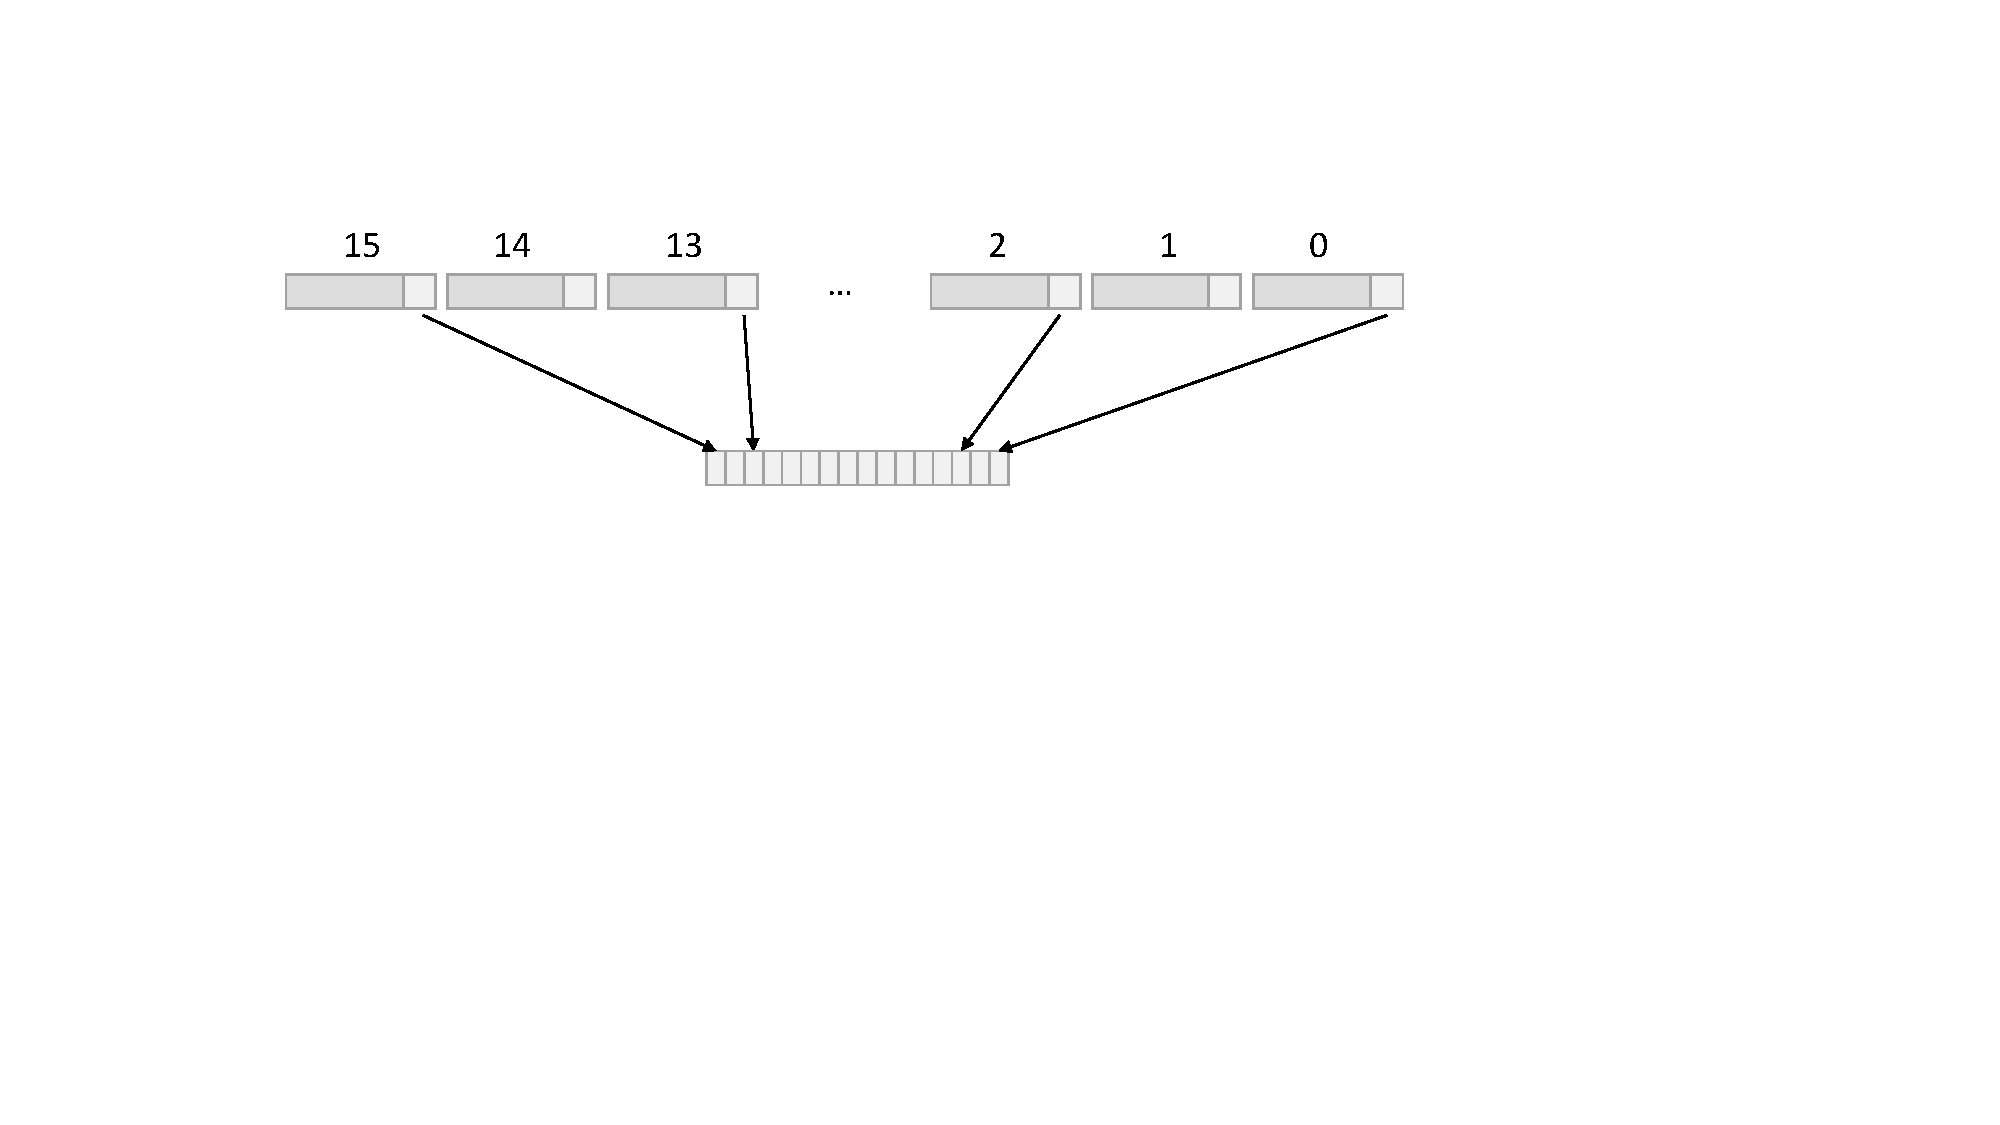
\includegraphics[height=3cm,trim={2cm 10.5cm 7cm 3cm},clip]{dgrm}
\caption{Diagram of the \texttt{\_mm\_movemask\_epi8} instruction mapping the LSB of 16 bytes to a 16 bit word.}
\end{figure}

This optimization was first observed in the cryptography community by the authors of the OT extension protocol~\cite{DBLP:conf/crypto/KellerOS15} and later described in a related work~\cite{DBLP:conf/ccs/KellerOS16}. While implementing this work and the related libOTe~\cite{libOTe} project, subsequently improved on this observation have been made. In particular, we employ Intel vector operations to allow 8  simultaneously\footnote{Most modern Intel CPUs support 8 vector lanes.} \texttt{\_mm\_movemask\_epi8} instructions to be performed, resulting in even greater throughput. In total these optimization represent several orders of magnitude improvement over a naive implementation and were essential in obtaining high performance.


Another computationally intensive operation is the construction of codewords that are subsequently secret shared. The most straight forward way to construct codewords $c\in\{0,1\}^n$ is by multiplying the the plaintext word $p\in\{0,1\}^m$ interpreted as a bit vector ($\mathbb{F}_2^n$) by a bit matrix $G\in\{0,1\}^{m\times n}$ known as the generator. Due to the code being linear, the result of this multiplication will be the desired codeword $c=Gp$. One important observation made by \cite{DBLP:conf/tcc/FrederiksenJNT16} is that a linear code can be placed in systematic form where codewords have the form $c=p||c'$, where $c'$ is a series of parity bit that can be computed with the generator matrix $G$. As such, only the parity bits $c'$ need be computing using matrix multiplication. However, this computation can still dominate the running time if implemented naively. Namely, the naive method is to test each bit of the input and then add the corresponding row of the generator matrix to a running sum if the bit is set. However, when performing this operations millions or more times, it can require significant time primarily due to the CPU not being able to effectively doing branch predication on the ``random" input bits, resulting in very poor instruction pipelining. 

Intuitively, we overcome this challenge by performing this conditional operation on a whole byte as opposed to single bits. This has several advantages: 1) fewer conditionals are performed. 2) branch prediction is not much more effective due to being conditioned on a whole byte.  3) The resulting operations can compatible with instruction vectorization. To enable this optimization, a pre-processing on the generator matrix $G$ is performed. $G$ is first decomposed into $G_1,...,G_{m/8}$ where $G_i$ is the $i$th set of 8 rows of the matrix $G$. For each $G_i$ and $s\in\mathbb{F}_2^8$, the value $G_is$ is computed and stored in a lookup table. Matrix multiplication by $G$ can then be reduced to
\[
   Gp = \sum_{i\in {1,...,m/8}} G_ip_i
\] 
,where $p_i$ is the $i$th set of 8 bits in $p$. When implemented, the right hand side can be efficiently instantiated as $m/8$ table lookups. The overhead of this approach is the initial pre-processing cost of generating the tables, consisting of $2^8$ matrix multiplications. However, when performing many commitments, this overhead is insignificant. To then achieve optimal performance, the table lookup operations can be vectorized, allowing 8 indexing operations to be performed in parallel. 

Our final optimization which is widely known in the cryptography community is the use of the AES-NI instruction set for performing fast pseudo-random number generation (PRNG). The implementation as is directly supports commitments on random values. These values are obtained by first performing $n$ so called base OTs on random and short strings. We then use these these short strings to generate the the two matrices of secret shared codeword. In particular, the base OTs are used as seeds to a PRNG. In all modern intel CPUs, the AES-NI instruction set allows for fast encryption via special hardware support. However, by placing AES in counter-mode, we can interpret it as a PRNG. As with the previous optimizations, it is critical for performance that these AES operations be vectorized, there at least 8 blocks of output are computed in parallel.
%In this section, we can share the insight that were gained from implementing it. This includes the SSE instructions for fast trnaspose. Your trick for doing the consistency check with mul128 instructions, and my fast linear code optimization.

In total, these optimizations improve the running time of the implementation by several orders of magnitude. When compared to the random oracle commitment scheme, where the computation is significantly more straight forward, these optimizations allow for an argument to be made that SplitCommit is an attractive alternative.